Figures~\ref{fig:Training_Flowchart_appendix} and \ref{fig:Inference_Flowchart_appendix}
show full-page vertical versions of the training and inference diagrams from the main text,
Figures~\ref{fig:Training_Flowchart} and \ref{fig:Inference_Flowchart}, respectively.

\clearpage

\section{Training Diagram}
Full-page vertical version of Figure~\ref{fig:Training_Flowchart}. See also
Figure~\ref{fig:Inference_Flowchart_appendix}.

\begin{figure}[p]
    \centering
    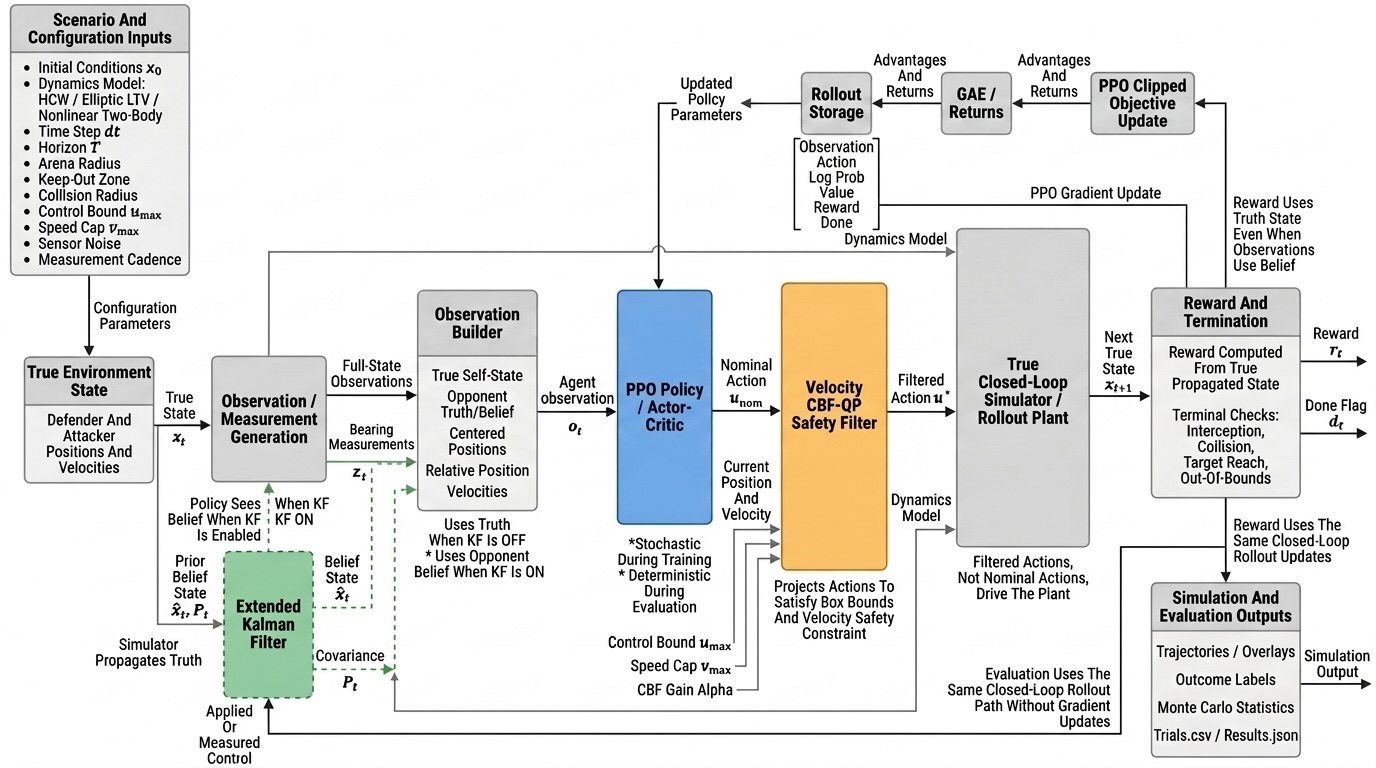
\includegraphics[angle=90,width=0.54\textheight]{Figures/Training_Improved_Flattened.jpg}
    \caption{Training diagram.}
    \label{fig:Training_Flowchart_appendix}
\end{figure}

\clearpage

\section{Inference Diagram}
Full-page vertical version of Figure~\ref{fig:Inference_Flowchart}. See also
Figure~\ref{fig:Training_Flowchart_appendix}.

\begin{figure}[p]
    \centering
    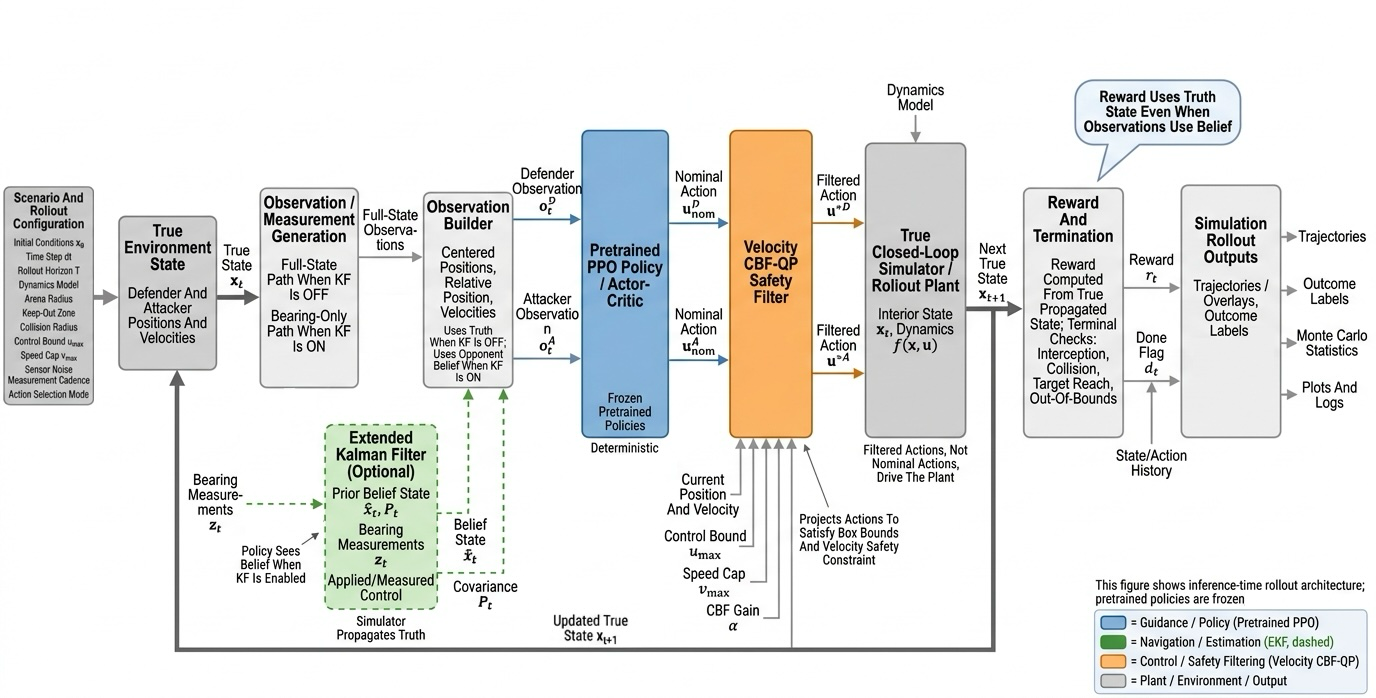
\includegraphics[angle=90,width=0.49\textheight]{Figures/Inference_Flattened.png}
    \caption{Inference diagram.}
    \label{fig:Inference_Flowchart_appendix}
\end{figure}

\clearpage